\documentclass[12pt]{article}
\usepackage[a4paper,margin=1in]{geometry}
\usepackage{setspace}
\usepackage{anyfontsize}
\usepackage{calc}
\usepackage{titlesec}
\usepackage[table]{xcolor}
\usepackage{booktabs}
\usepackage[font=scriptsize]{caption}
\usepackage{url}
\usepackage{latexsym}
\usepackage{graphicx}
\usepackage{amsmath}
 
\date{}

\begin{document}

\twocolumn[
\begin{center}
{\fontsize{12}{14}\selectfont\bfseries Real-Time Drone Sound Detection\par}

\vspace{1em}

\begin{tabular}{@{} c c @{}}
  {\fontsize{10}{12}\selectfont\bfseries Authors:\ 
     \normalfont\fontsize{9}{11}\selectfont Eduard Petrosyan, Ararat Kazarian} &
  {\fontsize{10}{12}\selectfont\bfseries Supervisor:\ 
     \normalfont\fontsize{9}{11}\selectfont Gagik Khalafyan} \\
  {\fontsize{9}{11}\selectfont\itshape BS in Data Science} &
  {\fontsize{9}{11}\selectfont\itshape AUA Adjunct Lecturer} \\
  {\fontsize{9}{11}\selectfont\itshape American University of Armenia} &
  {} \\
\end{tabular}

\vspace{1em}

{\fontsize{9}{11}\selectfont (Dated: May 9, 2025)\par}
\end{center}

% Abstract
\begin{center}
{\fontsize{9}{11}\bfseries Abstract}
\end{center}
\begin{center}
\begin{minipage}{0.95\textwidth}
\setstretch{1.1}
\setlength{\parindent}{1.5em}
{\fontsize{9}{11}\selectfont
The increasing use of small drones in modern warfare and civilian contexts has made them a decisive factor in both security and public safety. Due to their small size and ability to avoid radar detection, these drones are extremely difficult to detect using traditional methods. This project addresses this challenge by proposing an alternative method of drone detection based on sound. The focus is on developing a system that can detect and classify drone sounds in real-time using machine learning. 

A dataset of various environmental and drone-related sounds was used to train supervised learning models. Several classification algorithms were tested to identify the most accurate and efficient model for detecting UAV (Unmanned Aerial Vehicle) sound patterns. The chosen model was integrated into a working prototype capable of continuously analyzing audio input and detecting drone activity. 

This system can serve as a building block for broader applications such as autonomous threat detection systems, protection of sensitive facilities, smart surveillance in military zones, and monitoring of drone activity in urban or restricted areas. The prototype demonstrates the potential of sound-based methods as a valuable complement to existing detection technologies.

}
\end{minipage}
\end{center}

\vspace{2em} 
]

\begin{center}
{\fontsize{9}{11}\selectfont\bfseries I. INTRODUCTION} 
\end{center}

\vspace{0.5em}

{\fontsize{9}{11}\selectfont
In recent years, small drones have become prominent in both military and civilian contexts. On the battlefield, unmanned aerial vehicles (UAVs) are widely used for surveillance, target acquisition, and direct attacks. Kamikaze drones, designed to explode on impact, have turned drones into both reconnaissance tools and offensive weapons. In civilian settings, drones are increasingly used for commercial deliveries, aerial photography, and recreation—but they also pose risks when flown near restricted areas such as airports, government buildings, or critical infrastructure. Due to their compact size, many of these drones are difficult to detect with the naked eye, and their designs often reduce radar visibility, allowing them to bypass traditional detection systems and potentially threaten both military personnel and civilians.

Traditional drone detection relies heavily on visual tracking systems or radar technology. However, these methods often fail to identify small or low-flying drones, especially in cluttered or urban environments. This project addresses this challenge by proposing an alternative approach: real-time sound-based drone detection. Drones, even the quieter models, emit a distinct audio signature due to the rotation of their propellers. These audio patterns can be used to identify their presence before they are visible or picked up by radar.

The purpose of this project is to design and build a working prototype that uses machine learning to detect and classify drone sounds in real time. By analyzing environmental audio, the system can recognize specific drone-related sound patterns and trigger alerts. This kind of solution could be integrated into autonomous surveillance systems, used to protect critical infrastructure, monitor no-fly zones, or be deployed in conflict zones to improve situational awareness and save lives.

This work aims to show that sound can be a valuable and reliable signal for detecting threats in environments where other sensors might fail. The proposed system is not only affordable and practical but also adaptable to different use cases. It can be used to guard military bases, secure sensitive civilian areas such as airports or event venues, monitor restricted airspace, or support frontline operations. In situations where every second counts, having an early warning system based on audio can make a critical difference in preventing damage and saving lives.
    
}

\begin{center}
{\fontsize{9}{11}\selectfont\bfseries II. LITERATURE REVIEW}
\end{center}

\vspace{0.2em}

{\fontsize{9}{11}\selectfont
\indent In recent years, the field of audio classification has seen significant advancements, particularly with the integration of deep learning techniques. These developments have been driven by the need to accurately identify and classify various sound patterns in diverse environments. Key components contributing to these advancements include data augmentation methods, feature extraction techniques like Mel-Frequency Cepstral Coefficients (MFCCs) and mel-spectrograms, and the adoption of Convolutional Neural Networks (CNNs) for model training.

Data augmentation has emerged as a crucial strategy to enhance the performance of audio classification models, especially when dealing with limited datasets. Techniques such as time stretching, pitch shifting, adding Gaussian noise, and volume scaling have been employed to artificially increase the diversity of training data. These methods help models generalize better by simulating various real-world scenarios and recording conditions. A systematic review by Abayomi-Alli et al.\cite{abayomi2023augmentation} highlighted the effectiveness of these augmentation techniques in improving classifier robustness and performance across different sound classification tasks.

Feature extraction plays a pivotal role in transforming raw audio signals into representations suitable for machine learning models. MFCCs have been widely used due to their ability to capture the timbral aspects of audio signals, making them effective for tasks like speech and environmental sound recognition. Similarly, mel-spectrograms provide a time-frequency representation of audio, aligning closely with human auditory perception. A study by Iqbal et al.\cite{iqbal2021mel} demonstrated that models utilizing mel-spectrograms as input features achieved higher classification accuracy compared to those using traditional spectrograms, underscoring the importance of selecting appropriate feature representations.

The choice of model architecture significantly influences the success of audio classification systems. CNNs have been particularly effective in this domain due to their ability to learn hierarchical feature representations from input data. By treating mel-spectrograms as images, CNNs can exploit spatial hierarchies in the data, capturing both local and global patterns essential for accurate classification. Research by Palanisamy et al.\cite{palanisamy2024cnn} compared various CNN architectures and found that deeper networks with residual connections outperformed traditional models like K-Nearest Neighbors and Support Vector Machines, especially in complex audio classification tasks.

Integrating these components—robust data augmentation, effective feature extraction, and advanced CNN architectures—has led to significant improvements in audio classification performance. These methodologies collectively contribute to building systems capable of accurately detecting and classifying sounds in diverse and challenging environments.

}

\begin{center}
{\fontsize{9}{11}\selectfont\bfseries III. DATA}
\end{center}

\begin{center}
{\fontsize{9}{11}\selectfont\textit{1. Data Sources and Composition}}
\end{center}

\vspace{0.2em}

{\fontsize{9}{11}\selectfont
\indent The primary dataset utilized in this project is the DroneAudioDataset,\cite{AlEmadi2019Audio} a publicly available collection hosted on GitHub and developed as part of academic research into drone sound detection. This dataset is notable for its focus on the acoustic signatures of drones, providing short, labeled audio clips specifically curated for machine learning tasks in drone detection. The DroneAudioDataset includes recordings from two widely used commercial drones, the Parrot Bebop and Parrot Mambo, both individually and in mixed scenarios. These models are commonly encountered in both research and real-world environments, making the dataset highly relevant for practical applications. In total, the DroneAudioDataset comprises 1,332 drone audio clips and 10,372 non-drone audio clips, offering a substantial foundation for training and evaluating detection algorithms.

The drone audio was recorded in controlled indoor environments, capturing the propeller noise of the Bebop and Mambo drones during various flight conditions such as hovering and flying. The non-drone class was constructed from a diverse set of environmental sounds, including background noise, silence, and everyday activities, to ensure robust model generalization.

To further expand and balance the dataset, we developed a custom preprocessing utility that extracts one-second audio segments from longer video files, converting them into standardized .wav format. This approach enabled the generation of additional training samples from open-source sources, enhancing the dataset's diversity and real-world applicability.

In addition to the base DroneAudioDataset, both the drone and non-drone classes were enriched by incorporating audio samples from two major public sound libraries: Freesound.org\cite{freesound} and the BBC Sound Effects Archive\cite{bbc_sfx}. These sources contributed high-quality recordings of multirotor drones, flybys, and engine noises, as well as a broad spectrum of environmental background sounds such as traffic, indoor chatter, birdsong, and machinery. All collected audio was standardized to one-second clips and meticulously labeled prior to integration, ensuring consistency across the dataset.

\begin{table}[ht]
\centering
{\scriptsize
\rowcolors{2}{gray!10}{white}
\begin{tabular}{lrr}
\toprule
\rowcolor{gray!30}
Label & Raw Data & Augmented Data \\
\midrule
Drone      & 2,400  & 10,925 \\
Non-Drone  & 13,806 & 11,767 \\
\bottomrule
\end{tabular}
}
\caption{Number of audio samples per label before and after augmentation}
\label{tab:audio_label_counts}
\end{table}

The final raw dataset, summarized in Table~\ref{tab:audio_label_counts}, consists of 2,400 drone samples and 13,806 non-drone samples. This composition reflects an intentional class imbalance to mirror real-world conditions, where drone occurrences are relatively rare compared to everyday environmental noise. Data augmentation techniques were subsequently applied to address this imbalance and improve the robustness of the machine learning models.

}

\begin{center}
{\fontsize{9}{11}\selectfont\textit{2. Data Labeling, Preprocessing, and Augmentation}}
\end{center}

\vspace{0.2em}

{\fontsize{9}{11}\selectfont
\indent All audio samples were labeled for a binary classification task. Sounds produced by drones-including different models such as Bebop and Mambo, and regardless of the recording environment-were labeled as “drone.” All other sounds, including those from helicopters, vehicles, natural environments, and human activity, were labeled as “non-drone.” This binary framework reflects the primary goal of the system: to distinguish drone presence from all other auditory scenarios.

To ensure consistency, all audio files were resampled to a common sampling rate of 16,000 Hz. Recordings longer than one second were segmented into multiple one-second clips, while audio shorter than one second was excluded. This approach maintained uniform input lengths across all samples, which is essential for efficient model training.

For feature extraction, 13 Mel-Frequency Cepstral Coefficients (MFCCs) were computed from each one-second segment. MFCCs provide a compact and informative representation of the key audio characteristics necessary for classification. All features and their corresponding labels were saved in a compressed format for efficient loading during training.

To address the class imbalance observed in the raw dataset (see Table~\ref{tab:audio_label_counts}), data augmentation was applied specifically to drone audio segments. Techniques such as time stretching, pitch shifting, adding Gaussian noise, and volume scaling were used to create diverse variations of drone sounds. These transformations generated additional training examples, helping the model learn to recognize drones under a variety of acoustic conditions. Non-drone samples, which already encompassed a wide range of environmental sounds, were used without augmentation.

A mel-spectrogram visualization was created to illustrate the acoustic differences between the two classes. As shown in Figure~1, drone audio samples typically exhibit more regular and consistent frequency patterns, while non-drone samples display greater variation and irregularity.


\begin{figure}[ht]
\centering
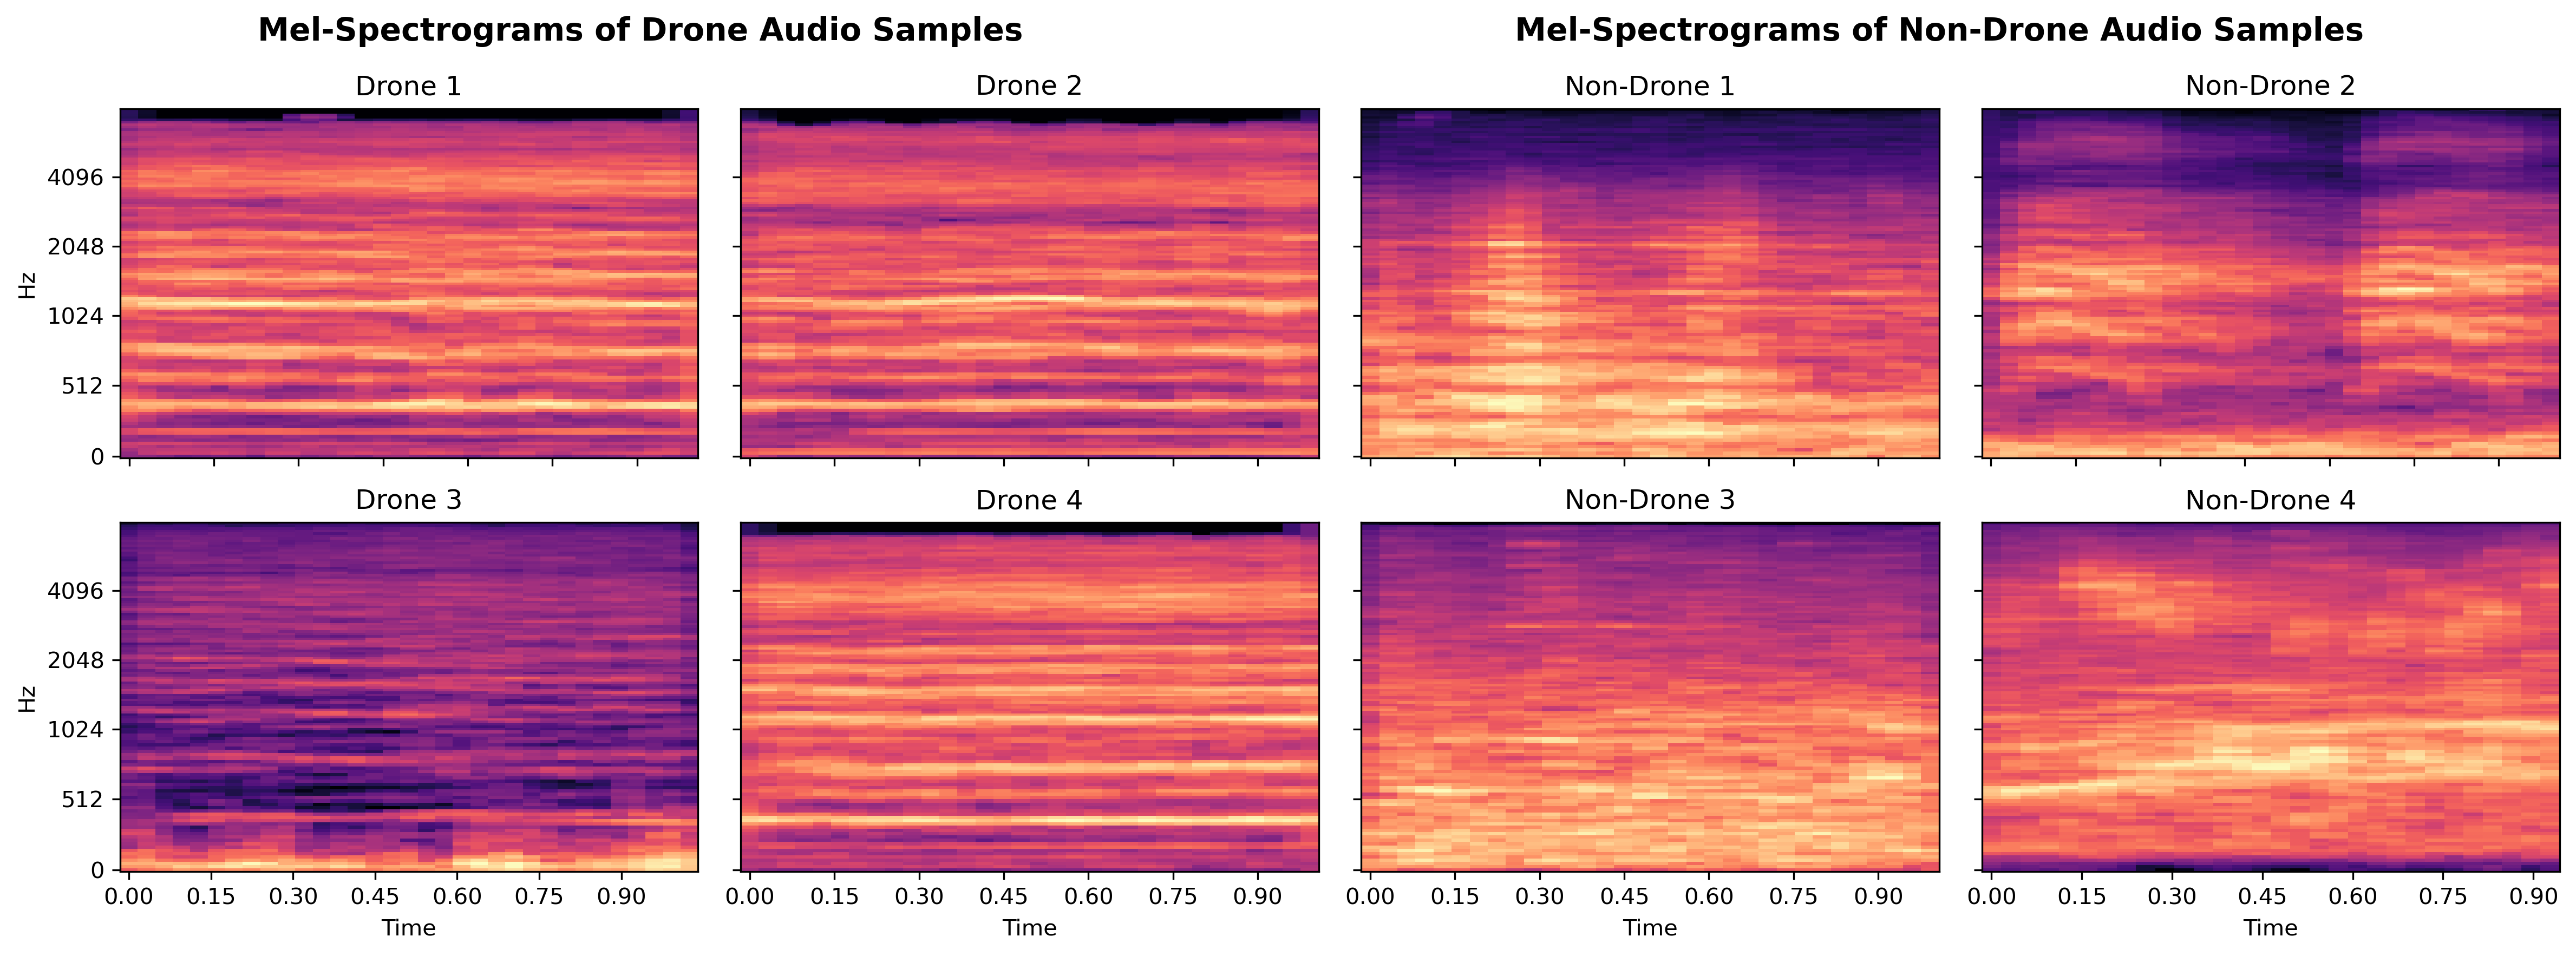
\includegraphics[width=\linewidth]{mel_spectrogram_comparison.png}
\caption{Mel-spectrograms of randomly selected drone and non-drone audio samples, illustrating characteristic frequency patterns.}
\label{fig:mel_spectrograms}
\end{figure}

After preprocessing and augmentation, the final dataset included 15,100 labeled one-second audio segments. The raw dataset, summarized in Table~\ref{tab:audio_label_counts}, originally contained 2,400 drone and 13,806 non-drone samples. Following segmentation and augmentation, the number of drone samples increased to 10,925, while the non-drone samples totaled 11,767. The total number of non-drone segments is slightly less than the original file count because audio clips shorter than one second were excluded, and some longer clips could not be divided into full one-second segments. The increase in drone samples is attributable to the data augmentation process, which generated additional variations from the original recordings.

}

\begin{center}
{\fontsize{9}{11}\selectfont\bfseries IV. METHODS}
\end{center}

\begin{center}
{\fontsize{9}{11}\selectfont\textit{1. Data Preparation}}
\end{center}

\vspace{0.2em}

{\fontsize{9}{11}\selectfont
All audio samples were preprocessed as described in Section III. After resampling, segmentation, and MFCC extraction, each one-second segment is represented by a \(32\times13\) feature matrix. The dataset was split 80/20 (stratified) into training and test sets. Data augmentation (time-stretch, pitch-shift, noise) was applied only to the drone class to correct class imbalance and improve robustness.

}

\begin{center}
{\fontsize{9}{11}\selectfont\textit{2. Model Selection}} 
\end{center}

\vspace{0.2em}

{\fontsize{9}{11}\selectfont
We evaluated six classifiers on the same MFCC features:
\begin{itemize}
  \item \textbf{K-Nearest Neighbors (KNN)} — an instance-based method that assigns each segment the majority label among its $k$ nearest neighbors in MFCC space. It’s simple, interpretable, and works well when classes form compact clusters, but can degrade if noise causes feature overlap.
  \item \textbf{Logistic Regression} — a linear model that predicts the probability of “drone” vs. “non-drone” via a logistic function. This serves as a strong baseline, especially when the two classes are roughly linearly separable in feature space.
  \item \textbf{Support Vector Machine (SVM)} — learns a maximum-margin hyperplane (optionally via kernels) to separate classes. It handles high-dimensional MFCC inputs robustly and can model non-linear boundaries with kernels like RBF.
  \item \textbf{Random Forest} — an ensemble of decision trees built on bootstrap samples. By aggregating many trees, it captures non-linear dependencies among MFCC features and is naturally robust to noisy or irrelevant features.
  \item \textbf{XGBoost} — a gradient-boosted tree ensemble that iteratively fits trees to the residuals of previous models. It often achieves state-of-the-art performance on tabular features, handles class imbalance well, and can model complex decision boundaries.
  \item \textbf{Convolutional Neural Network (CNN)} — learns hierarchical spectro-temporal filters from the raw MFCC matrices. By applying 2D convolutions, it can pick up local patterns (e.g., propeller harmonics) more effectively than “flat” feature-based learners.
\end{itemize}

For some non-CNN models, hyperparameter tuning was performed using methods best suited to the characteristics of each algorithm, while others were retained with default settings due to satisfactory baseline performance. Specifically, for logistic regression, five-fold cross-validation was employed to select the optimal regularization parameter and prevent overfitting. For K-Nearest Neighbors, we plotted test accuracy against different values of $k$ (number of neighbors) and selected the value that yielded the highest validation accuracy. For the remaining models-Support Vector Machine, Random Forest, and XGBoost-the default hyperparameters provided strong baseline results on our dataset and were therefore retained without further tuning.

}

\begin{center}
{\fontsize{9}{11}\selectfont\textit{3. Model Evaluation}}
\end{center}

\vspace{0.2em}

{\fontsize{9}{11}\selectfont
We measure accuracy and F1-score on the held-out test set (Table~\ref{tab:model_results}). Although XGBoost slightly outperformed the CNN numerically, we chose the CNN for deployment because:
\begin{enumerate}
  \item Its convolutional layers exploit local time–frequency patterns in MFCCs (e.g. propeller harmonics).
  \item It generalizes better to unseen acoustic variations.
  \item Inference on modern edge hardware can be extremely fast, enabling real-time continuous monitoring.
\end{enumerate}

}

\begin{table}[ht]
\centering
{\scriptsize
\rowcolors{2}{gray!10}{white}
\begin{tabular}{lcc}
\toprule
\rowcolor{gray!30}
\textbf{Model} & \textbf{Accuracy} & \textbf{F1-Score} \\
\midrule
K-Nearest Neighbors      & 0.970 & 0.970 \\
Logistic Regression      & 0.889 & 0.889 \\
Support Vector Machine   & 0.970 & 0.970 \\
Random Forest            & 0.980 & 0.980 \\
XGBoost                  & 0.983 & 0.983 \\
CNN                      & 0.971 & 0.971 \\
\bottomrule
\end{tabular}
}
\caption{Test set accuracy and F1-score for all evaluated models.}
\label{tab:model_results}
\end{table}

\begin{center}
{\fontsize{9}{11}\selectfont\textit{4. Convolutional Neural Network}}
\end{center}

\vspace{0.2em}

{\fontsize{9}{11}\selectfont
To effectively capture the distinctive spectrotemporal characteristics of drone and non-drone audio, we developed a compact Convolutional Neural Network (CNN) tailored for efficient classification of MFCC-based features. The input to the network is a $32 \times 13$ matrix, where 32 represents the number of time frames and 13 is the number of Mel-Frequency Cepstral Coefficients extracted from each one-second audio segment. This representation preserves both the temporal and spectral information necessary for distinguishing drone sounds from a wide variety of environmental noises.

The CNN architecture is intentionally streamlined to facilitate real-time processing and minimize computational overhead. It begins with a two-dimensional convolutional layer consisting of 16 filters of size $5 \times 5$, followed by a ReLU activation and a $2 \times 2$ max pooling operation. This initial stage enables the network to learn local time-frequency patterns that are characteristic of drone acoustics. The resulting feature maps are then flattened and passed through two fully connected layers: the first with 64 units and ReLU activation, and the second producing class logits for the binary classification task.

This simple yet effective architecture was chosen to ensure low inference latency, making it highly suitable for deployment on resource-constrained hardware such as embedded systems or edge devices. By limiting the depth and parameter count of the network, we significantly reduce both computational complexity and memory requirements, which is critical for applications that demand real-time or near-real-time response. Despite its simplicity, the CNN demonstrated robust performance in both controlled experiments and field tests, effectively discriminating between drone and non-drone sounds even in the presence of background noise.

The use of MFCCs as input further enhances the model’s robustness and efficiency, as these features provide a compact and perceptually meaningful summary of the audio signals. Overall, this CNN-based approach offers an optimal balance between accuracy, efficiency, and deployability, enabling practical, real-time drone detection in diverse operational environments.

}

\begin{center}
{\fontsize{9}{11}\selectfont\textit{5. Real-Time Processing}}
\end{center}

\vspace{0.2em}

{\fontsize{9}{11}\selectfont
To demonstrate the practical utility of our drone detection system, we developed a real-time processing application with an intuitive graphical user interface (UI). The application is designed to operate on a standard notebook or desktop computer, utilizing the built-in microphone as its audio input source.

Upon launch, the application continuously captures audio data from the microphone in one-second chunks. Each audio segment undergoes the same preprocessing pipeline as described in previous sections, including resampling, segmentation, and extraction of 13 Mel-Frequency Cepstral Coefficients (MFCCs). These features are then fed into the trained Convolutional Neural Network (CNN) model, which classifies the input as either "drone" or "non-drone" in real time.

A key feature of the UI is the dynamic visualization of the Mel-spectrogram for each processed audio segment. The Mel-spectrogram is displayed prominently, providing users with an immediate visual representation of the frequency content and temporal evolution of the captured sound. This not only enhances transparency but also aids in understanding the acoustic patterns associated with drone activity.

The user interface is organized into two main sections below the spectrogram display. The first section presents the probability score for the presence of a drone, while the second section shows the probability for non-drone sounds. These probabilities are updated every second, reflecting the model’s real-time confidence in its predictions. This dual-indicator approach allows users to quickly assess the likelihood of drone activity at any given moment.

\begin{figure}[ht]
\centering
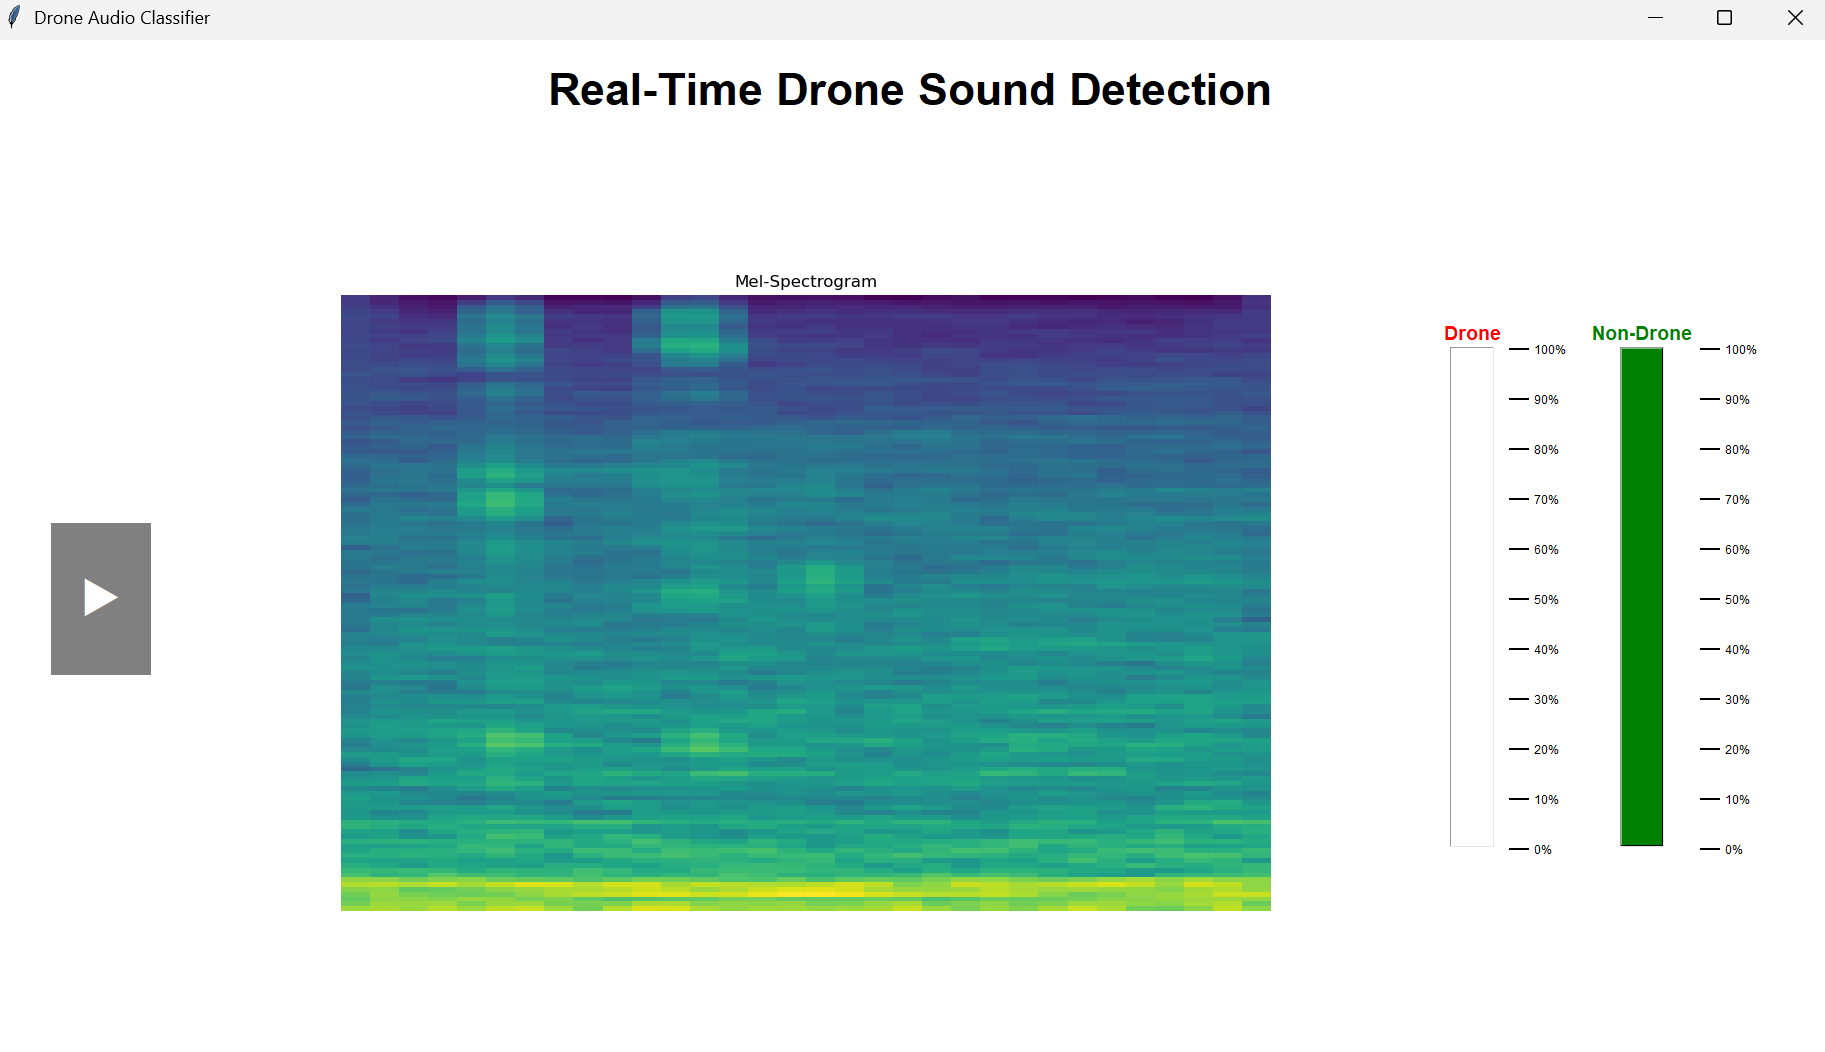
\includegraphics[width=\linewidth]{ui.png}
\caption{The user interface of the application in real time. The visualization of the Mel-spectrogram is shown in the center, and real-time probability indicators for the classification of drones and non-drones are displayed next to it.}
\label{fig:mel_spectrograms}
\end{figure}

Overall, the real-time application provides an accessible and informative interface for drone sound detection. By combining visual feedback with probabilistic outputs, it enables both technical users and non-experts to monitor and interpret drone activity efficiently and effectively.

}

\begin{center}
{\fontsize{9}{11}\selectfont\bfseries V. FINDINGS}
\end{center}

\vspace{0.2em}

{\fontsize{9}{11}\selectfont
\indent The real-time drone detection application developed in this project demonstrated strong performance in practical field testing. During evaluation at the 
Azatazen Polygon field, the system was able to reliably detect the sound of an FPV drone from a distance of approximately 30-40 meters. Detection remained consistent within this range, even under typical outdoor noise conditions. These results indicate that the proposed sound-based approach is effective for real-time UAV monitoring in open environments. It is important to note that the detection range could be further increased by employing higher-quality or more sensitive microphones, suggesting potential for even broader deployment in real-world scenarios.

}

\begin{center}
{\fontsize{9}{11}\selectfont\bfseries VI. CONCLUSION }
\end{center}

\vspace{0.2em}

{\fontsize{9}{11}\selectfont
\indent This work presented a comprehensive approach to drone sound detection using machine learning and real-time audio processing. By leveraging a diverse dataset, advanced data augmentation, and a convolutional neural network model, the system achieved robust performance in both controlled and field conditions. The real-time prototype successfully identified drone activity at significant distances, demonstrating the practical value of audio-based detection methods as a complement to traditional surveillance technologies. Future improvements, such as integrating higher-grade microphones and expanding the dataset with more drone types and environments, could further enhance detection accuracy and operational range.

}


\begin{center}
{\fontsize{9}{11}\selectfont\bfseries VII. FUTURE PLAN}
\end{center}

\vspace{0.2em}

{\fontsize{9}{11}\selectfont
\indent As this project was developed as a prototype, several realistic improvements can be made to continue its development at the student level or in collaboration with local organizations.

One of the immediate next steps is to test the system in more realistic environments within Armenia. For example, drone sound detection could be tested near schools, public events, or university campuses where drones might be present either recreationally or for filming purposes. This would help assess how well the system distinguishes drone sounds from ambient urban noise and other common background activity.

Another practical improvement would be to design a small portable device using affordable components like a basic microcontroller and a microphone. This would allow the model to be tested in outdoor conditions without relying on a full computer setup. Students could experiment with open-source platforms like Arduino or Raspberry Pi to achieve this.

Additionally, the model could be improved by recording more drone sounds under different conditions in Armenia, such as windy weather, mountainous areas, or urban canyons where echo and noise may interfere with audio clarity. Collaborating with local drone hobbyist groups or the AUA Drone Club could help gather these sound samples and increase dataset diversity.

A longer-term goal might be to explore partnerships with civic organizations or municipalities to pilot the system in specific areas where drone monitoring is relevant—for example, near national heritage sites or events where drone use is restricted.

Looking ahead, we also hope to establish contact with Armenian national security institutions and propose a collaboration to simulate a controlled battlefield-like acoustic environment. Such a simulation would help us evaluate the detector’s performance under realistic conflict conditions, including overlapping noises, varied terrain, and potential drone swarming. This could serve both as a research opportunity and as a practical contribution to national security by offering early-stage support for passive drone detection systems.

These future directions aim to gradually evolve the project from a university prototype into a more field-ready system, with improvements driven by local needs, low-cost experimentation, and collaboration within the community.

}

\begin{center}
{\fontsize{9}{11}\selectfont\bfseries VIII. ACKNOWLEDGMENTS}
\end{center}

\vspace{0.2em}

{\fontsize{9}{11}\selectfont
\indent We express our sincere gratitude to our supervisor, Gagik Khalafyan, for his professional guidance, insightful feedback, and consistent support throughout the development of this project. His mentorship helped us navigate challenges, structure our work effectively, and refine our approach with clarity and purpose.

We also extend our heartfelt thanks to the AUA Drone Club for their valuable assistance during the testing phase of our system. Their support included access to relevant drone equipment, particularly an FPV (First-Person View) drone, help with setting up test scenarios, and technical expertise that contributed to the reliable evaluation of our prototype. Their collaboration was instrumental in testing the system under realistic conditions and ensuring the functionality of our solution.

Finally, we would like to thank the American University of Armenia for providing a supportive academic environment and access to the necessary resources and infrastructure that made this project possible.

}

\onecolumn
\vspace{1em}

{\fontsize{7.5}{9}\selectfont
\bibliographystyle{plain}
\bibliography{Bibliography}
}

\end{document}
